\chapter{Results \& Discussion}\label{c:results}
In the following sections, parts of the sensor subsystems are analyzed and the results obtained from dew point measurement shown and discussed. 

\section{Sensor subsystems}


\subsection{Temperature readout}

The temperature readout is among the most critical parts of the sensor system, as the temperature has to be determined as an absolute value with sufficient accuracy. Hence, an early test was the evaluation of multiple temperature sensors to evaluate suitable candidates for usage on the platform. Besides accuracy, critical parameters are also defined to be drift and response time, as the measurement principle requires correctness over an extended time period as well as a sufficiently fast response to temperature gradients.



The first sensor board included tests over five different temperature and ambient conditions sensors. It was performed using a Fluke 5615 \gls{SPRT}, specifying an accuracy of \qty{\pm 0.012}{\celsius} and an extremely low drift of \qty{\pm 0.007}{\celsius} at the triple point of water (\qty{0.01}{\celsius}). Therefore, its specified accuracy is approximately an order of magnitude higher than that of the tested integrated temperature sensors and hence it may be used as a reference for accuracy measurements. For the temperature control, a Fluke 7320 calibration bath was used, inside which the temperature sensors were submerged in a low viscosity silicon oil. This allows for very fine control and uniformity in temperature within the measurement environment. 

\begin{wrapfigure}{r}{0.55\textwidth}
    \centering
    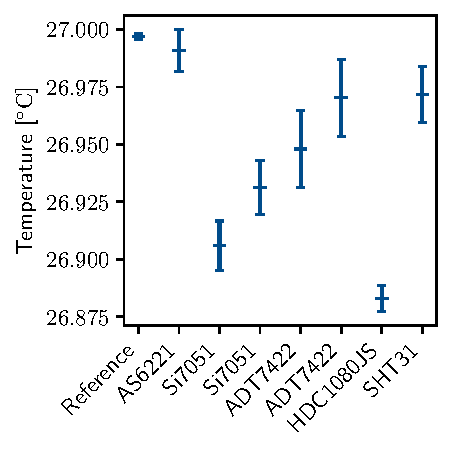
\includegraphics{graphs/tempsensors_stability.pdf}
    \caption{Long duration test of temperature sensors at \qty{27}{\celsius}.}
    \label{g:temp_stability}
\end{wrapfigure}
The readout of the temperature sensors was performed in cycles of \qty{200}{\ms} using a microcontroller, which sent its data to a host machine. The \gls{SPRT} was measured using 4-wire measurement on a Keysight 3458A multimeter in order to eliminate voltage drop on the lead wires and the data was fetched over serial communication in the same frequency as for the integrated temperature sensors. The conversion from resistance to temperature was performed using the supplied ITS-90 calibration coefficients, which were specified around 2.5 years prior to measurement and state an uncertainty of around \qty{\pm 10}{\milli\kelvin} at \qty{0.01}{\celsius}. Although the drift is not specified in datasheet, it is assumed to be as low as \qty{\pm 1}{\milli \kelvin} per year, as related studies show \autocite{tavenerPlatinumResistanceThermometers2013}. The accuracy of the resistance measurement of the multimeter is stated with approximately \qty{\pm 15}{ppm} for the respective range of \qty{100}{\kilo\ohm} and the calibration period of two years, resulting in a temperature deviation of less than \qty{5}{\milli \kelvin}.

\begin{figure}[t!]
    \centering
    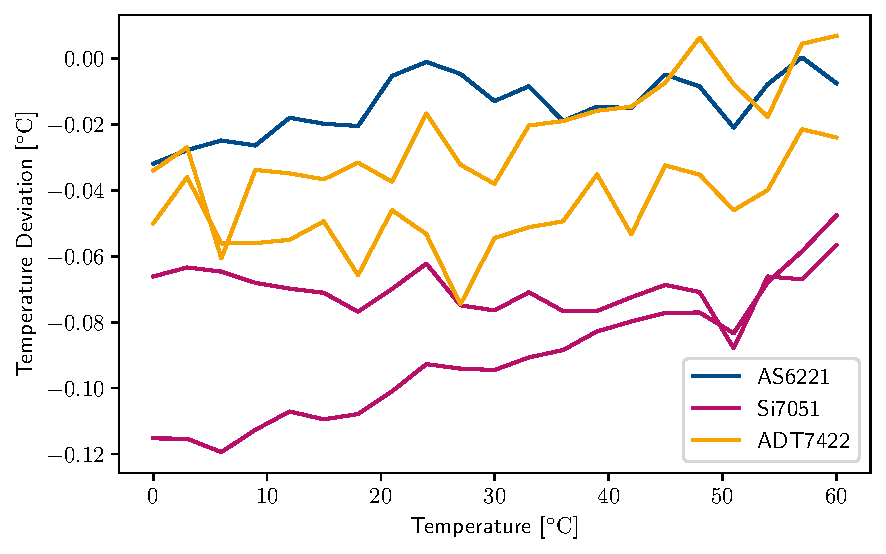
\includegraphics{graphs/tempsensors_dev.pdf}
    \caption{Temperature deviations for each sensor compared to the \gls{SPRT}.}
    \label{g:temp_dev}
\end{figure}

\Cref{g:temp_stability} shows the deviations during a long duration measurement of 30 minutes. The sensors used for the test were primarily the later used ams-OSRAM AS6221, Silicon Labs Si7051 and Analog Devices ADT7422. Although two samples of each sensors were intended to be tested, a mechanical failure led to one AS6221 sensor to be dismissed in the analysis. Two results of two additional humidity and temperature sensors (Texas Instruments HDC1080JS and Sensirion SHT31) have been included as well. The results show the mean temperature measurement of each sensor, as well as the standard deviation. As expected, the \gls{SPRT} showed the smallest amount of variation with around \qty{\pm 3}{\milli\celsius}. While the HDC1080JS follows right after that with around \qty{\pm 8}{\milli\kelvin}, it has the largest deviation in the absolute measurement, indicating less trueness. Hence, for this test the AS6221 sensor is determined to be the most accurate among the sensors, as it is closest to the measurement of the \gls{SPRT} while showing relatively low variations.

Another test is shown in \cref{g:temp_dev}, comparing the sensors over a range of different temperatures. For each sensor and temperature, 20 samples were taken and their mean value compared against the reference temperature reading of the \gls{SPRT}. Again, the AS6221 showed the least deviation with a maximum of \qty{-35}{\milli\celsius} at \qty{0}{\celsius}.

Besides the superior performance in temperature measurement, the AS6221 sensor also exhibits the lowest response time after a rapid change in temperature. This can be explained by its low thermal mass, as it is the smallest sensor of all, with a footprint size of \qtyproduct{1 x 1.5}{\mm}.


\subsection{Temperature control}
The temperature control is another important subset of the humidity sensor. A precise control is necessary in order to avoid measurement inaccuracies due to oscillation in temperature or changing temperature gradients.

The performance is mainly decided by two factors, the buck converter being able to supply sufficient power for the \gls{TEC} and the \gls{PID} controller, which is governing the output voltage of the buck converter.

The buck converter was designed with high current application in mind. It uses rather large \qty{330}{\milli\henry} inductance rated for \qty{3.5}{\ampere}, thus requiring \qtyproduct{12.5 x 12.5}{\mm} \gls{PCB} area. Due to the high inductance however, switching frequencies can be limited to less than \qty{200}{\k\Hz} without large sacrifices in terms of ripple, limiting the dissipated heat of the device. During tests it was found, that the buck converter is capable to provide sustained currents as high as \qty{3.5}{\A} at around \qty{14}{\V}, which is sufficient for a temperature difference of \qty{40}{\celsius}.

\begin{figure}[!b]
    \centering
    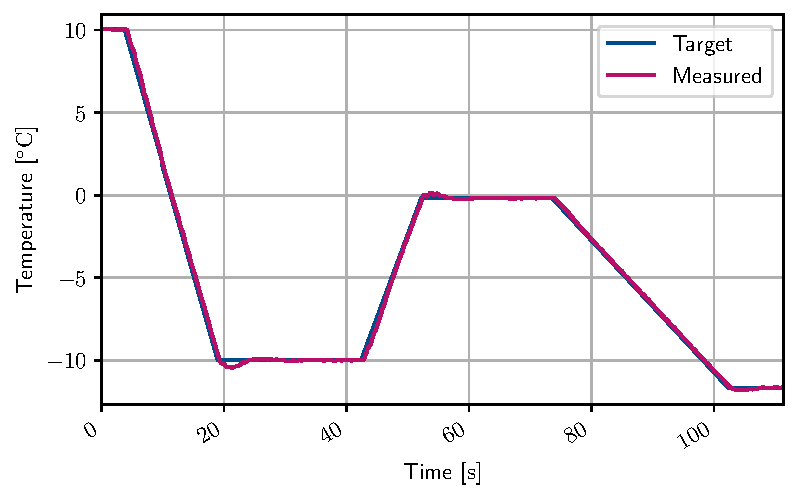
\includegraphics{graphs/pid_offset.pdf}
    \caption{Comparison of set temperature and measured temperature in a simulated dew point measurement scenario.}
    \label{g:pid}
\end{figure}

The \gls{PID} controller uses proportional, integral and derivative error terms for feedback as explained in \cref{c:implementation}. In order to find a suitable initial set of coefficients, the Ziegler-Nichols method was used. It is an heuristic approach, using the period of oscillations in a purely proportianally controlled system in order to define the integral and derivative terms. From there on, further manual adjustments have been made to optimize the performance. Main concern for the system is a high degree of linearity in order to avoid unstable dew formation and noise in temperature measurement. \Cref{g:pid} shows a resulting temperature control in an environment with starting conditions of \qty{10}{\celsius}. Beginning from t = \qty{4}{\s}, the temperature slopes have been set to \qty[per-mode=fraction]{-1.3}{\celsius\per\s} until \qty{-10}{\celsius} is reached, \qty[per-mode=fraction]{0}{\celsius\per\s} for \qty{23}{\s}, \qty[per-mode=fraction, retain-explicit-plus]{+1}{\celsius\per\s} until \qty{0}{\celsius} is reached, \qty[per-mode=fraction]{0}{\celsius\per\s} for \qty{21}{\s} and \qty[per-mode=fraction]{-0.4}{\celsius\per\s} for \qty{94}{\s}. The measured values follow the setpoint line closely, with very little difference in terms of slope. Only in case of a rapid change in the temperature set point slope, there is a clearly visible oscillation. To avoid these oscillations, the system would require either a decrease in the integral term or an increase in the derivative term, however, this would come at the cost of increased offsets, or respectively oscillations, during constant slope operation.


\subsection{Optical and capacitive readout}
The optical and capacitive readout need to reliably measure the presence of dew on the surface. In contrast to the temperature sensor, the measure quantity does not need to be detected as an absolute value, e.g. as gram or volumetric ratio, but as a relative value compared to the initial state of the system. Hence, most important factors of the dew detection are considered to be sensitivity and noise behaviour.

\subsubsection{Capacitor}
The sensitivity of the capacitive readout is first and foremost limited by the resolution of the frequency measurement of the capacitor, given that a change in capacitance is detected by the charging and discharging time of the component. This results in a proportionate relation to the product of the charge-discharge period and the sampling frequency. In the context of the measurement system, this means, the resistor governing the current and thus the period needs to be sufficiently large, while sampling with a high frequency. 

The used values were set to  \qty{1}{\mega\ohm} for the resistor and \qty{170}{\mega\Hz} for the frequency, being the maximum possible frequency for the microcontroller. The value of the capacitor was determined to be around \qty{180}{\pico\F}. At operating voltages of \qty{3.3}{\volt} for the supply voltage and measured threshold voltages of \qty{1.05}{\volt} and \qty{1.55}{\volt}, this results in a period of $T_{RC} = \qty{115.34}{\us}$ or a frequency of \qty{8.67}{\kilo\Hz} using \cref{e:cap_period}, given standard ambient conditions and neglecting stray capacitances. With a sampling period of $T_{s} = \frac{1}{\qty{170}{\mega\Hz}} = \qty{5.88}{\ns}$, this results in a sensitivity of around \qty{51}{ppm}. 

However, this high amount of sensitivity is severely limited by noise introduced into the measurement system. The noise sources affecting the system are countless, among these are:
\begin{itemize}
    \item fluctuations in supply voltage
    \item fluctuations in threshold voltage
    \item fluctuations in sampling frequency
    \item electromagnetic interference
    \item temperature
    \item mechanical forces
\end{itemize}

\begin{wrapfigure}{r}{0.5\textwidth}
    \centering
    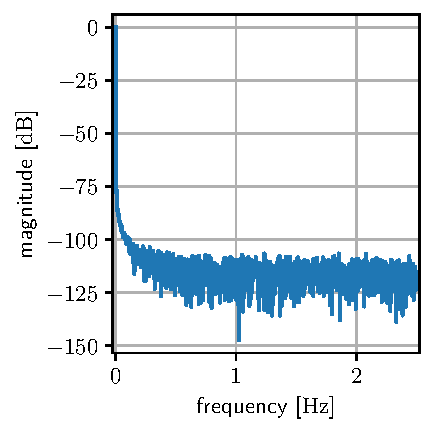
\includegraphics{graphs/noise_cap.pdf}
    \caption{Noise analysis of capacitor readout.}
    \label{g:noise_cap}
\end{wrapfigure}
Some of these influences may be minimized by design or changes in the measurement environment, while others are given. Noise estimation is a rather difficult task due to measured size, i.e. water concentration in close proximity to the surface, being noisy. \Cref{g:noise_cap} shows a \gls{FFT} of a measurement cycle with a duration of 10 minutes, with samples taken every \qty{200}{\ms}. At higher frequencies, the Fourier transform looks flat, resembling the power spectrum of white noise, while the frequency response in the lower section follows a pink noise pattern. The measurements were conducted in controlled conditions, which were yet not completely constant with an approximately linear change in temperature of \qty[retain-explicit-plus]{+50}{\milli\celsius} and a relative humidity change of \qty[retain-explicit-plus]{-0.05}{\percent}, as measured using four temperature and three humidity sensors. The measured frequency of the Schmitt trigger circuit exhibits a response closely following the linear trend detected by the other sensors, with the frequency rising linearly from \qtyrange{6270}{6290}{\Hz}.

High noise influences on the measurement are evident however when the \gls{TEC} is powered during sensing of the capacitor, with standard deviations one order of magnitude higher than without, rendering reliable capacitance measurements infeasible. Therefore during all capacitive measurements, the \gls{TEC} is turned off. Furthermore, the capacitive readout uses 20 samples, in order to determine and remove outliers, and uses an average of the remaining values in order to reduce the impact of high frequency noise.


\subsubsection{Optical readout}
The optical readout relies on the precision of the used proximity sensors. Both are specified to detect objects within a range of \qty{20}{\mm}, yet their difference different light source leads to a different output code for a given distance. The configuration of the sensors has been set such, that their output uses as much of the scale as possible. The VNL36825T, employing a laser that emits a much narrower beam of light, uses nearly the full scale of 16 bit, with values ranging between 40000 and 60000 during the performed humidity measurements. The VCNL4040 sensor is only able to provide values that are a factor 10 lower.

\begin{figure}[!hb]
    \centering
    \begin{subfigure}{.5\textwidth}
      \centering
      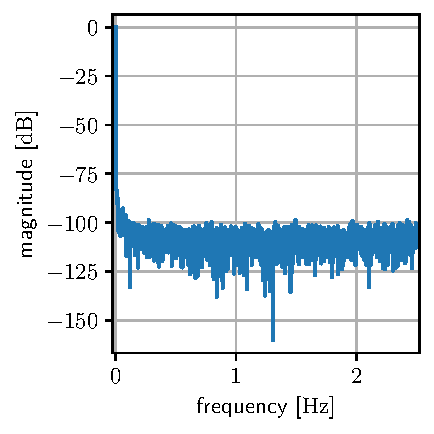
\includegraphics{graphs/noise_prx1.pdf}
      \caption{VCNL4040}
      \label{g:noise_prx1}
    \end{subfigure}%
    \begin{subfigure}{.5\textwidth}
      \centering
      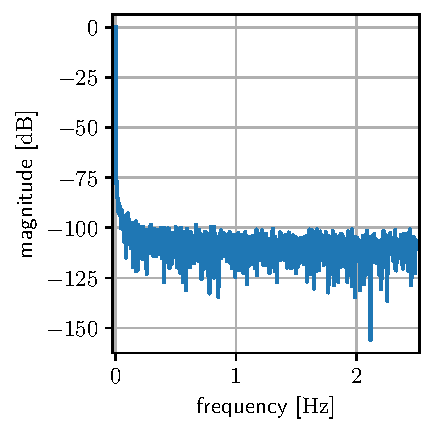
\includegraphics{graphs/noise_prx2.pdf}
      \caption{VCNL36825T}
      \label{g:noise_prx2}
    \end{subfigure}
    \caption{Noise analysis of the two center proximity sensors.}
    \label{g:noise_prx}
\end{figure}


\section{Humidity measurements}

\subsection{Test setup}
The hygrometric measurements were performed within an environment where conditions were regulated to maintain maximal stability. This required careful considerations for the test setup, which was established as seen in \cref{d:test_chamber}. 

The desired temperature conditions were achieved using a temperature test chamber, which is roughly sealed with some cables leaving a millimeter-sized gap to the outside. Inside the test chamber, a sealed box is placed, which is prepared with thoroughly sealed cable glands. This box contains the hygrometer, which is placed on top of a perforated plate. Below the perforated plate is a screw glass containing the reference humidity solution. For proper air exchange, such that the desired humidity can easily be reached, a fan has been put on top of the glass. For cooling of the peltier element, a heatsink and another fan was used.

\begin{figure}[h]
    \centering
    \input{drawings/test_setup.pdf_tex}
    \caption{Test chamber setup.}
    \label{d:test_chamber}
\end{figure}

The tests have been performed for three temperature and four saturation vapor pressure setpoints, which are defined by the respective substance as seen in \cref{t:equi}. The substances are mixed with water such that the water is saturated, with sufficient amount of the unsolved substance being able to draw moisture from the air. In order to reach saturation for a given temperature, the test chamber was first set to the respective target temperature with a maximum deviation of \qty{\pm0.1}{\celsius} as measured by the integrated temperature sensors. If the temperature conditions were stable, there was a settling period of \qtyrange{2}{3}{h} in order to guarantee saturation. The state was also observed using the reference humidity sensors such that no significant changes in relative humidity were observable. The sensor was tried to be left without modification, however due to increased requirements for cooling at lower temperatures, the thermal paste connecting the heatsink to the \gls{FPC} was replaced, leading to differences in absolute values of measured frequency and light. As the dew point is performed using relative changes, these changes are assumbed to be minor in terms of humidity detection. The measurements performed using the changed conditions are indicated by an asterisk at the respective rows of \cref{t:equi}.

% \begin{wraptable}{l}{1\textwidth}
\begin{table}
        \centering
    \begin{tabular}{r|ccccc|c}
        \toprule
        \toprule
    Substance                        & T [\unit{\celsius}] & RH [\unit{\percent}] & Deviation & AH [\unit{\g\per\m^3}] & p [\unit{\hecto\Pa}] \\
    \midrule
    \multirow{3}{*}{MgCl\textsubscript{2}}           & 10          & 33.47                      & \textpm 0.24 &       3.16 &       4.13 & *\\
    & 25          & 32.78                      & \textpm 0.16 &       7.59 &      10.44  & *\\
    & 40          & 31.60                      & \textpm 0.13 &      16.23 &      23.45  & \\
    \midrule
    \multirow{3}{*}{Mg(NO\textsubscript{3})\textsubscript{2} * 6H\textsubscript{2}O} & 10          & 57.36                      & \textpm 0.33 &       5.42 &       7.08  & *\\
    & 25          & 52.89                      & \textpm 0.22 &      12.25 &      16.85  & \\
    & 40          & 48.42                      & \textpm 0.37 &      24.87 &      35.94  & \\
    \midrule
    \multirow{3}{*}{NaCl}            & 10          & 75.67                      & \textpm 0.22 &       7.15 &       9.34  & *\\
    & 25          & 75.29                      & \textpm 0.12 &      17.43 &      23.99  & \\
    & 40          & 74.68                      & \textpm 0.13 &      38.35 &      55.43  & \\
    \midrule
    \multirow{3}{*}{K\textsubscript{2}SO\textsubscript{4}}           & 10          & 98.18                      & \textpm 0.76 &       9.27 &      12.12  & *\\
                                     & 25          & 97.59                      & \textpm 0.53 &      22.59 &      31.09  & \\
                                     & 40          & 96.71                      & \textpm 0.38 &      49.67 &      71.78  & \\
                                     \bottomrule
    \end{tabular}
    \caption{Equilibrium relative humidities of the substances used for measurement. Measurements performed using a change in the setup are marked by an asterisk.}
    \label{t:equi}
\end{table}
% \end{wraptable}


\subsection{Initial measurements}

\begin{figure}[h]
    \centering
    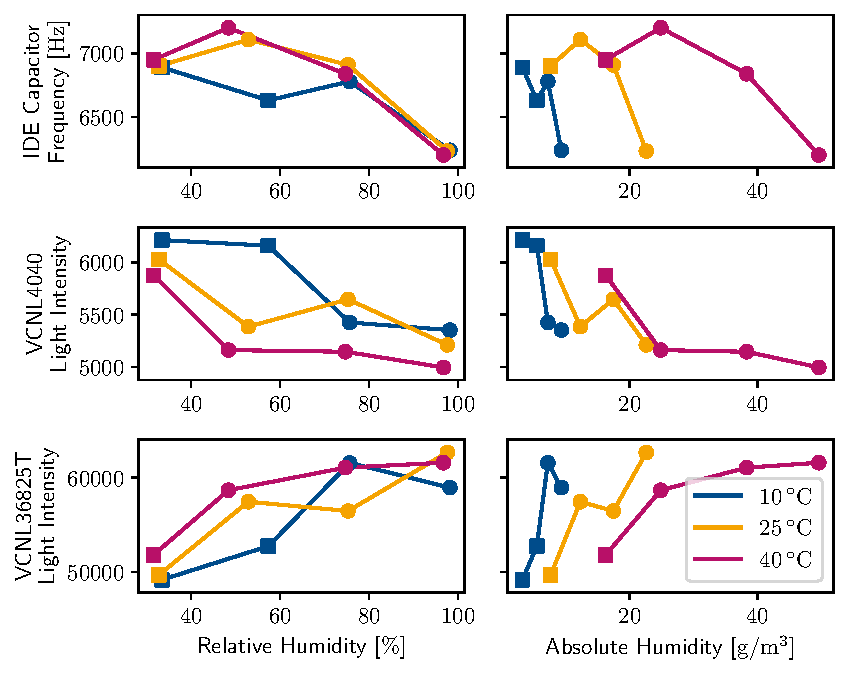
\includegraphics[width=1\textwidth]{graphs/start_range_cap_light.pdf}
    \caption{Measurements taken at the beginning of the cycle.}
    \label{g:initial_measurements}
\end{figure}

Each measurement cycle begins with a short duration for data collection in order to set thresholds based on the starting condition in order to limit cooling duration. \Cref{g:initial_measurements} shows the inital readout values at the start of the measurement cycle for each temperature as well as for each relative and absolute humidity. The circled data points were taken from a measurement before the changes on the cooling system, the rectangular data points were taken afterwards, hence any comparison between these two data series in terms of absolute values must be taken with care. Nonetheless the diagrams show a clear dependence of the initial reading on both temperature and humidity. Especially in terms of relative humidity (as seen on the left), there is a clear proportional relationship within the samples of each data series, suggesting the possibility to make qualitative predictions on relative humidity prior exact dew point determination. Correspondingly, the relation of the frequency and the absolute humidity is much less pronounced, e.g. resulting in a frequency of \textgreater\qty{7200}{\Hz} and \textgreater\qty{6200}{\Hz} for and approximate absolute humidity of \qty{20}{\g\per\m^3} at \qty{25}{\celsius} and \qty{40}{\celsius} respecively. 

With decreasing water vapor pressure however, the difference in readings between different ambient temperatures becomes less significant, with the data points being horizontally (yet also vertically) closer together at smaller absolute humidity values. This result is consistent with the behaviour of certain types of integrated capacitive humidity sensors. Chen and Jin proposed a porous $\alpha$-alumina sensor chip, which features a thin anodic-spark-deposited $\alpha$-Al\textsubscript{2}O\textsubscript{3} film with a thickness of \qty{5}{\um}, which is capable of sensing absolute humidty between dew point temperatures of \qtyrange{-80}{-10}{\celsius} and relative humidity in a range of \qtyrange{10}{95}{\percent} RH \autocite{chenAlphaaluminaMoistureSensor1992}.

The light sensors show likewise a proportional behaviour along the relative humidity values. The slopes are inverse however, possibly indicating that the photodiode of the VCNL36825T receives an increased amount of light due to the scattering.

% Capacitive sensors using porous films work on two principles of adsorption, chemisorption and physisorption. Chemisorption is a process in which a chemical reaction occurs between the surface and the adsorbate, resulting in the formation of new chemical bonds at the adsorbent surface. This process is highly selective and occurs only when a chemical connection with the adsorption site is possible; if it is, the chemisorbed complex forms the first immobile and potentially irreversible layer. As such it is also an important factor in long term drift, as the the porosity and surface area changes. In contrast, physisorption is a process in which the adsorbate and the surface remain intact and are held together by weak intermolecular van der Waals forces. The first physisorbed layer is 

\subsection{Dew point measurements}

\begin{figure}[h!]
    \centering
    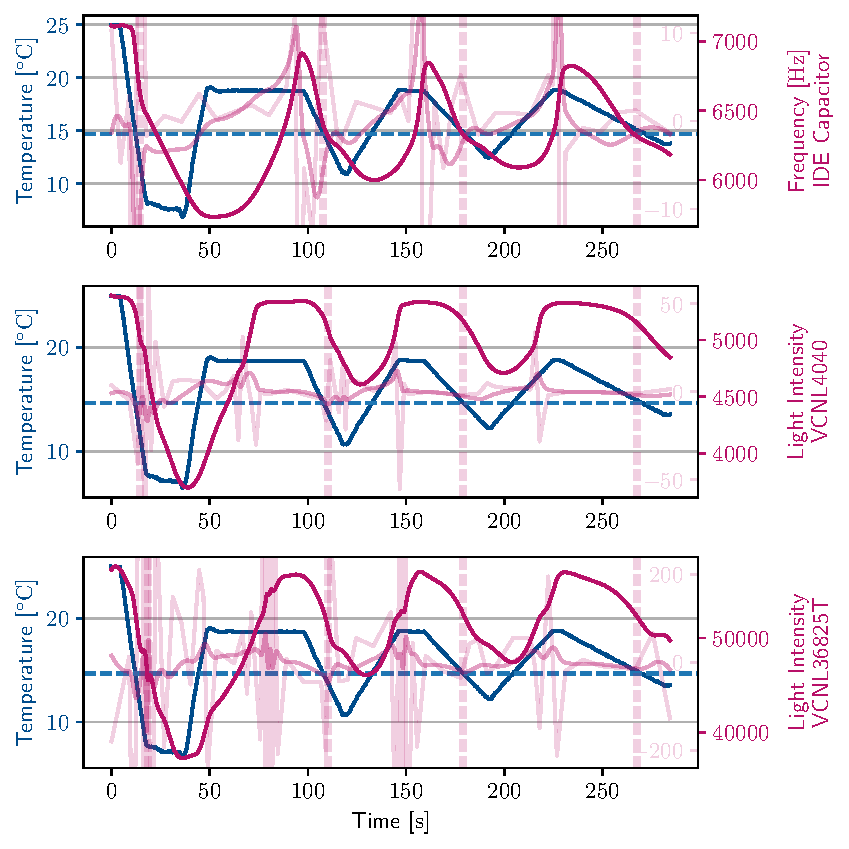
\includegraphics{graphs/measurementT25RH50.pdf}
    \caption{Measurement cycle at T = \qty{25}{\celsius} and RH = \qty{52.89}{\percent}. The opaque solid lines show the temperature and the regression curve of the sensor reading respectively. The transparent lines show the derivatives of the regression curve, with the darker line being the first and the lighter line being the second derivative. The reference dew point is indicated with the blue dashed lines and the dew point detection indicated by the transparent red dashed lines.}
    \label{g:meas_cycle}
\end{figure}
The actual dew point measurements are performed as described in \cref{c:control,c:readout}. The measurement cycle is set to four decreasing and three increasing slopes with $s = \{ \qty[per-mode=fraction]{-1.3}{\celsius\per\s}, \qty[per-mode=fraction, retain-explicit-plus]{+1}{\celsius\per\s}, \qty[per-mode=fraction]{-0.4}{\celsius\per\s}, \qty[per-mode=fraction, retain-explicit-plus]{+0.3}{\celsius\per\s},\qty[per-mode=fraction]{-0.2}{\celsius\per\s}, \qty[per-mode=fraction, retain-explicit-plus]{+0.2}{\celsius\per\s},\qty[per-mode=fraction]{-0.1}{\celsius\per\s} \}$. The first decrease is used in order to set temperature targets for subsequent cooling using a percentage of the measured frequency of the capacitor as the controlling threshold. As during the first decrease in temperature, the response time of the mirror/capacitor surface is larger, as well as due to the threshold required to be set suffieciently low, there is a large error in this first realtime dew detection. This offset is compensated by adding a sufficiently large positive offset, such that the range for successive heating and cooling cycles is set to be between the detected temperature at the threshold and a positive offset of \qty{10}{\celsius}. 

\Cref{g:meas_cycle} shows an exemplary measurement cycle at an initial temperature of T = \qty{25}{\celsius} and a relative humidity of RH = \qty{52.89}{\percent}. In the following it serves as an example to describe the dew point detection algorithm. During a decrease in temperature, the measured values decrease, indicating a increased capacitance measurement for the capacitor and and an increase in scattering for the proximity sensors. The amount of the decrease per time step rises at first, although with a slight temporal offset, especially for the first period. However, at a certain point, there is a slight step in the measured curve. Here, visible amount of dew starts to form, leading to a direct change in the response of the respective sensors. The difficulty in the measurement lies in the temporal offset however. 

The capacitive sensor is much more responsive, hence the change is sensed the earliest among all sensors. The proximity sensors exhibit a certain amount of lag. Aggravating is the fact, that this temporal response is related to the slope of the temperature curve. For small changes in temperature over time, the step appears at a later moment in time and with a temperature gradient set too low, the step cannot reliably detected at all, as seen in the last period of the VCNL4040 dew point detection.

Due to this, the dew point detection of the proximity sensors has been set to an earlier point in time, namely the point, where the second derivation of the sensed value is minimal, or in other words, where the decrease in temperature accelerates most. For all sensors an additional offset of 10 samples has been chosen in order to provide guidance and to show potential benefits in further offset consideration.

\Cref{t:dew_points} show the resulting dew point values in comparison with the reference value. Due to time constraints a complete depiction over all measurements could not be performed and remains topic for further work. For the graphical representation of all measurements please refer to \cref{appendix}.

\begin{table}[]
    \begin{tabular}{|r|clllllll|}
    \hline
    Sensor     & \multicolumn{2}{c|}{Period 1}                           & \multicolumn{2}{l|}{Period 2}                           & \multicolumn{2}{l|}{Period 3}                           & \multicolumn{2}{l|}{Period 4}      \\ \hline
    Capacitor  & \multicolumn{1}{c|}{13.23} & \multicolumn{1}{l|}{10.98} & \multicolumn{1}{l|}{15.25} & \multicolumn{1}{l|}{14.41} & \multicolumn{1}{l|}{15.08} & \multicolumn{1}{l|}{14.72} & \multicolumn{1}{l|}{15.11} & 14.92 \\ \hline
    VCNL4040   & \multicolumn{1}{c|}{13.23} & \multicolumn{1}{l|}{10.98} & \multicolumn{1}{l|}{14.34} & \multicolumn{1}{l|}{13.48} & \multicolumn{1}{l|}{15.08} & \multicolumn{1}{l|}{14.72} & \multicolumn{1}{l|}{15.11} & 14.92 \\ \hline
    VCNL36825T & \multicolumn{1}{c|}{8.41}  & \multicolumn{1}{l|}{8.2}   & \multicolumn{1}{l|}{14.34} & \multicolumn{1}{l|}{13.48} & \multicolumn{1}{l|}{15.08} & \multicolumn{1}{l|}{14.72} & \multicolumn{1}{l|}{15.11} & 14.92 \\ \hline
    Reference  & \multicolumn{8}{c|}{14.72}                                                                                                                                                                                       \\ \hline
    \end{tabular}
    \label{t:dew_points}
    \caption{Measured dew points for each sensor for the example given in \cref{g:meas_cycle}.}
    \end{table}


\subsection{Discussion}
The dew point analysis is a complicated topic requiring precise measurements. \Cref{acceptable_error} shows the maximum allowed deviations in dew point measurement in order to achieve a \qty{1}{\percent} accuracy over a range of temperatures and humidities. Higher temperatures and humidities have a larger amount of acceptable error, while for high humidity measurements in low temperatures, the acceptable error becomes close to zero.  
\begin{figure}[h]
    \centering
    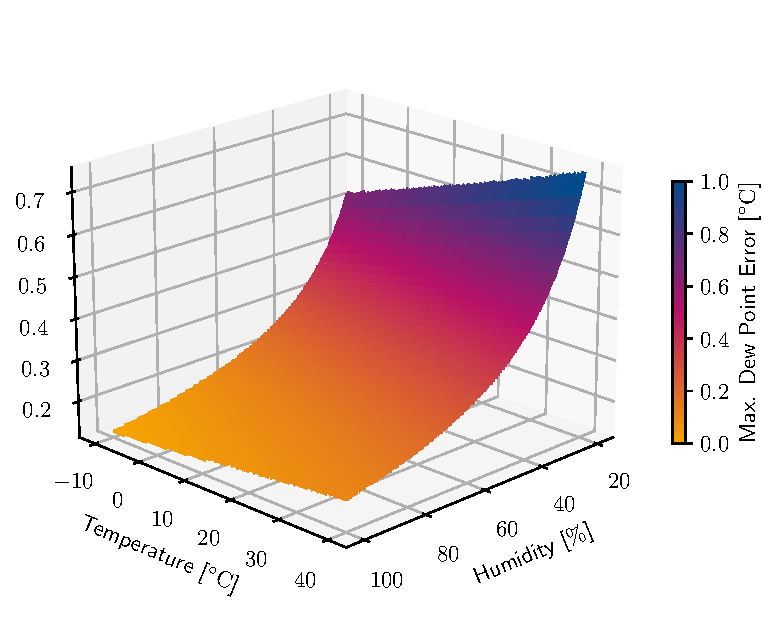
\includegraphics[clip, trim=0cm 0cm 0cm 1cm, width=0.95\textwidth]{graphs/dew_deviation.pdf}
    \caption{Maximum Dew Point Temperature Tolerance for a \qty{1}{\percent} accuracy}
    \label{acceptable_error}
\end{figure}